\usepackage[authoryear,round]{natbib}
\newcommand{\sheetnum}{%
	02
}
%\setcounter{section}{\sheetnum-3}
\newcommand{\tutorialtitle}{%
    Connectionist Neuron \& Function Fitting
}
\newcommand{\tutorialtitleshort}{%
	Perceptron \& Learning
}
% for slides
\subtitle{\sheetnum \tutorialtitle}

\maxdeadcycles=1000 % Workaround for ! Output loop---100 consecutive dead cycles because of too many figures

% The following use of algroithms does not work well with the notes:
%
%
%
%
% instead use the following for your algorithms:
%
%\begin{figure}[!t]
%\removelatexerror
%\begin{algorithm}[H]
    % your aglo here
    %\label{alg:algolabel}
    %\caption{algocaption}
%\end{algorithm}
%\end{figure}
%\begin{algorithm}
% Below is the definition for the command \removelatexerror:
\makeatletter
\newcommand{\removelatexerror}{\let\@latex@error\@gobble}
\makeatother{}

\begin{document} %%%%%%%%%%%%%%%%%%%%%%%%%%%%%%%%%%%%%%%%%%%%%%%%%%%%%%%

\maxdeadcycles=1000 % Workaround for ! Output loop---100 consecutive dead cycles because of too many figures

\sheet{\sheetnum}{\tutorialtitleshort}

\ttopic{\tutorialtitle}

\columnratio{0.2,0.8}\textbf{}
\begin{paracol}{2}
%\setlength{\columnseprule}{0.1pt}
%\setlength{\columnsep}{5em}

\begin{rightcolumn}

% notes version will ignore it
\begin{frame}
\titlepage
\end{frame}

\begin{frame}{The plan for today}
\tableofcontents
\end{frame}

%\mode<all>
%\input{./0_connectionist_neuron}
%\mode*

%\clearpage

%\mode<all>
%\section{Limitations of Perceptrons}

\mode<presentation>{
\begin{frame} 
    \begin{center} \huge
        \secname
    \end{center}
    \begin{center}
    From neurons to neural networks
    \end{center}
\end{frame}
}

\mode<article>{
Connectionist neurons, or perceptrons, are limited in the variety of functions they are able to fit. 
When dealing with classification problems, a perceptron can only find a linear separation between any two classes. Irrespective of the neuron's non-linear activation function, the perceptron is regarded as a \emph{linear classifier}. Whether something falls on one side of the decision boundary or the other, is entirely based on applying a linear filter (i.e. $\vec w^{\top} \vec x$). The non-linearity $f(h)$ merely controls the value range of the neuron's response ($\{0,1\}, (-1,+1)$, \ldots) which helps in interpreting the neuron's response.\\

If observations for two different classes are distributed such that one cannot draw a line to separate them, then the two classes
are not linearly separable. In this case, the perceptron will fail to find a suitable classification boundary between the two classes.
}

\begin{frame}\frametitle{Linear classifiers/linear decision boundaries}

Consider the following binary classification problems with $\vec x \in \R^2$.{}

\question{Can you find a line that separates the two classes for each case?}

\begin{figure}[h]
    \centering
	\includegraphics[width=0.8\textwidth]{img/and_or_xor_y}
	\mode<article>{
	\caption{(a) points are classified according to the AND function,
	(b) points are classified according to the OR function,
	(c) points are classified according to the XOR function.
	}
	}
	\label{fig:and_or_xor} 
\end{figure}

\mode<article>{
In \figureref{fig:and_or_xor}, particularly (a) and (b),
it is possible to draw a line that separates the classes. Therefore, the AND and OR functions are linearly separable.
A perceptron is capable of finding such a separating line. However, this does not apply to the third case, for the XOR function.
It is impossible to find a single line that will separate the classes.\\
The XOR function is not linearly separable.
}

\pause 

\question{Can we solve the XOR problem with multiple perceptrons? How?}\\

%\slidesonly{
%\begin{figure}[ht]
     %\centering
	%\includegraphics[trim=480 0 0 30, clip, width=0.4\textwidth]{img/and_or_xor_y.png}
	%\caption*{A single perceptron can not solve the XOR problem.}
	%\label{fig:xor} 
%\end{figure}
%}

\pause

\notesonly{
- Yes, think of it as a divide and conquer approach. We split the XOR problem into multiple sub-problems. 
A perceptron is used to solve each sub-problem.

If you're familiar with Boolean algebra, you might recognize the following expression for the XOR function:
}
\mode<presentation>{
\vspace{-10mm}
}

\begin{equation}
\label{eq:xor}
\mathrm{XOR}(x_1, x_2) = 
({\color{magenta}\,{x_1} \; \mathrm{AND} \; \overline{x}_2 \,})
 \;\; \mathrm{OR} \;\; 
({\color{green}\, \overline{x}_1 \; \mathrm{AND} \; x_2 \,})
\end{equation}

\end{frame}

\begin{frame}{Inversion/NOT-Gate}

\begin{center}
\begin{minipage}{0.9\textwidth}

\begin{center}
\begin{minipage}{0.45\textwidth}
	\includegraphics[width=0.9\textwidth]{img/neuron_3d_grid_hyperplane}
\end{minipage}
\begin{minipage}{0.45\textwidth}
	\includegraphics[width=0.9\textwidth]{img/neuron_3d_grid_hyperplane_flip}
\end{minipage}

\end{center}
\end{minipage}
\captionof{figure}{Inverting a neuron's response by flipping the hyperplane}
\end{center}

\end{frame}


\mode<article>{
For instance, the first perceptron ${\color{magenta}s^1_1}$ is tasked to separate the bottom-right cloud of points from the rest. 
A second perceptron ${\color{green}s^1_2}$ is used to separate the top-left cloud from the rest.
A third perceptron ${\color{blue}s^2_1}$ will then use the responses of both and respond to ``is \textbf{only one} of the two perceptrons \textbf{on}?''.

\figref{fig:build_xor} illustrates this approach. One need only recognize that each sub-problem is linearly separable.\\
}

\begin{frame}

\slidesonly{
\begin{equation}
\label{eq:xor}
\mathrm{XOR}(x_1, x_2) = 
({\color{magenta}\,{x_1} \; \mathrm{AND} \; \overline{x}_2 \,})
 \;\; \mathrm{OR} \;\; 
({\color{green}\, \overline{x}_1 \; \mathrm{AND} \; x_2 \,})
\end{equation}
}

\begin{figure}[ht]
    \centering
	\includegraphics[width=0.75\textwidth]{img/build_xor_crf}
	\caption{Solving sub-problems of the XOR problem.}
	\label{fig:build_xor} 
\end{figure}

\end{frame}

\begin{frame}

\begin{figure}[ht]
    \centering
	\includegraphics[width=0.75\textwidth]{img/build_xor}
	\caption{Solving sub-problems of the XOR problem.}
	\label{fig:build_xor} 
\end{figure}

\end{frame}


\mode<article>{
\figref{fig:xor_decisions} visualizes the response of the final neuron $s^2_1$ for different values of $x_1$ and $x_2$. The space is partitioned into one region in which the activity is $< 0.5$ and two disjoint regions (top-left \& bottom-right) in which the activity is $> 0.5$.
}

\begin{frame}
\begin{figure}[ht]
     \centering
     \savebox{\imagebox}{
     \mode<presentation>{
	 \includegraphics[width=0.4\textwidth]{img/xor_decision}
	 }
     \mode<article>{
	 \includegraphics[width=0.35\textwidth]{img/xor_decision}
	 }
	 }%
     \begin{subfigure}[t]{0.35\textwidth}
         \centering
         \usebox{\imagebox}% Place largest image
         \caption{}
         \label{fig:xor_decisions}
     \end{subfigure}
     \slidesonly{
     \hspace{4mm}
     \begin{subfigure}[t]{0.45\textwidth}
     }
    \notesonly{
     \hspace{1mm}
     \begin{subfigure}[t]{0.38\textwidth}
     }
         \centering
         \raisebox{\dimexpr.5\ht\imagebox-.5\height}{% Raise smaller image into place
         \includegraphics[width=0.9\textwidth]{img/xor_decision_s}
         }
         \caption{}
         \label{fig:xor_decisions_s}
     \end{subfigure}
	\caption{Identifying the decision boundaries.}
\end{figure}
\end{frame}

\newpage
\mode<article>{


What we are essentially describing is a Multilayered perceptron (MLP) with an architecture as illustrated in \figref{fig:xor_mlp_arch}. This MLP is made up of an output layer with a single output neuron ${\color{blue}s^2_1}$, and one hidden layer with two hidden neurons, ${\color{magenta}s^1_1}$ and ${\color{green}s^2_2}$ (the superscript denotes the layer index, the subscript denotes the neuron index within its layer). The terms ``neurons'' and ``nodes'' are treated as synonyms.
}
\begin{frame}

\begin{figure}[ht]
    \centering
	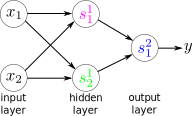
\includegraphics[width=0.4\textwidth]{img/xor_mlp_arch}
	\caption{simplified MLP architecture}
	\label{fig:xor_mlp_arch} 
\end{figure}



\end{frame}



%\mode*

%\newpage

\mode<all>
\section{Ingredients for function fitting}

\mode<presentation>{
%\begin{frame}{Where are we?}
%\begin{columns}
    %\begin{column}{0.55\textwidth}
        %\tableofcontents[currentsection,hideallsubsections]
    %\end{column}
    %\begin{column}{0.45\textwidth}
        %\begin{center}
            %\includegraphics[width=0.8\textwidth]{img/meme_ingredients}
        %\end{center}
        %\begin{center}
        %Tuning the weights of a model to perform some task.
        %\end{center}
    %\end{column}
%\end{columns}
%\end{frame}
\begin{frame}
    \begin{center} \huge
        \secname
    \end{center}
    \begin{center}
        \includegraphics[width=0.4\textwidth]{img/meme_ingredients}
    \end{center}
    \begin{center}
        Tuning the weights of a model to perform some task.
    \end{center}
\end{frame}
}

\begin{frame}\frametitle{\secname}

    \mode<article>{
    Fitting a model to a desired function $y(\vec x)$ requires the following:
    }

    \begin{enumerate}
    \item<1-> 
    \mode<article>{A cost function  with the objective to optimize it, often a minimization problem:}
    \mode<presentation>{A cost function:\vspace{-10mm}}
	\begin{equation}
		e\tyxw \eqexcl \min_{\vec w}
	\end{equation}
    \item<2-> A performance measure, a criterion for \emph{model selection}.
    \mode<article>{Specifically, \\

    the generalization \textbf{error} $E^G$ which is defined as:}	
    \begin{equation} 
                \EGw \; := \; \left<\,e\,\right>_{y_T, \vec{x}; \vec w} 
                \; = \; \iint d \vec{x} \, dy_T \; 
                    P{(y_T, \vec{x})} \, e{\tyxw}
    \end{equation}
    \only<2>{
    Because $P{(y_T, \vec{x})}$ is not known, \mode<article>{we turn to the principle of empirical risk minimization (ERM).
    According to ERM we can approximate $\EGw$ by computing the} empirical average $\ETw$ using the available training data:
    $$
    \left\{\left(\vec x^{(\alpha)}, y_T^{(\alpha)}\right)\right\}, \alpha=1,\ldots,p
    $$.
    \mode<article>{The training error $\ETw$ becomes:}

    \mode<presentation>{\vspace{-10mm}}
    }
    \begin{equation}
    \only<2>{
    \text{batch training error:}\quad}\ETw=\frac{1}{p}\sum_{\alpha=1}^{p} \underbrace{e\tyxwalpha}_{e^{(\alpha)}}
    \end{equation}
    \mode<article>{
    where $e\tyxwalpha$ (or $e^{(\alpha)}$ for brevity) is the cost computed from the prediction for a specific observation $y(\vec x^{(\alpha)};\vec w)$ and its corresponding label $y_T^{(\alpha)}$. The superscript $^{(\alpha)}$ is used to index a specific point (sample) in the dataset.
    }
    \item<3-> A model with tunable parameters $\vec w$: connectionist neuron, MLP,\ldots
    \item<4-> A learning algorithm\mode<article>{ for finding the set of parameters in our model that will minimize the cost function.\\
    This can be done analytically (depending on some conditions) or through an iterative learning algorithm (e.g. gradient-based learning)}
    \end{enumerate}

\end{frame}


\mode*

\newpage

\mode<all>
\input{./3_cost}
\mode*

\clearpage

\mode<article>
\subsection{From KL-divergence to the cross-entropy cost in numbers}

\subsubsection{First: The KL-divergence in numbers}

\definecolor{darkgreen}{rgb}{0,0.6,0}
\begin{align}
\dkl&\left(\, P_{\text{data}}(\vec x, y) \,||\, P_{\text{model}}(\vec x, y) \,\right)\\
&= \underbrace{
	\int_{\R^N} d \vec x \,
	{ \color{darkgreen} P_{\text{data}}(\vec x) }
	\sum_{y \in \{\textcolor{red}{0},\textcolor{blue}{1}\}}
	P_{\text{data}}(y | \vec x)
	\ln 
	\lbrack { \color{violet} P_{\text{data}}(y | \vec x) } \rbrack
	}_{\text{indep. of } \vec w~\Rightarrow~\text{treat as const. =}~c} \\
	&\qquad- \int_{\R^N} d \vec x \,
		{ \color{darkgreen} P_{\text{data}}(\vec x) }
			\sum_{y \in \{\textcolor{red}{0},\textcolor{blue}{1}\}}
			P_{\text{data}}(y | \vec x)
			\ln
			\lbrack {\color{brown} P_{\text{model}}(y | \vec x) } \rbrack\\
&= c \; - \int_{\R^N} d \vec x \,
		{ \color{darkgreen} P_{\text{data}}(\vec x) }
			\sum_{y \in \{\textcolor{red}{0},\textcolor{blue}{1}\}}
			P_{\text{data}}(y | \vec x)
			\ln
			\lbrack {\color{brown} P_{\text{model}}(y | \vec x) } \rbrack\\
&= c \; - \int_{\R^N} d \vec x \,
		{ \color{darkgreen} P_{\text{data}}(\vec x) }
		\Big\lbrack
			P_{\text{data}}(\textcolor{red}{y=0} | \vec x)
			\ln
			\lbrack {\color{brown} P_{\text{model}}(\textcolor{red}{y=0} | \vec x) } \rbrack\\
	&\qquad\qquad\qquad\qquad +
			P_{\text{data}}(\textcolor{blue}{y=1} | \vec x)
			\ln
			\lbrack {\color{brown} P_{\text{model}}(\textcolor{blue}{y=1} | \vec x) } \rbrack
		\Big\rbrack\\
&= c \; - \int_{\R^N} d \vec x \,
		{ \color{darkgreen} P_{\text{data}}(\vec x) }
			P_{\text{data}}(\textcolor{red}{y=0} | \vec x)
			\ln
			\lbrack {\color{brown} P_{\text{model}}(\textcolor{red}{y=0} | \vec x) } \rbrack\\
	&\qquad- \int_{\R^N} d \vec x \,
		{ \color{darkgreen} P_{\text{data}}(\vec x) }
			P_{\text{data}}(\textcolor{blue}{y=1} | \vec x)
			\ln
			\lbrack {\color{brown} P_{\text{model}}(\textcolor{blue}{y=1} | \vec x) } \rbrack
\end{align}

\begin{enumerate}
\item \textbf{Correctly} classifiying a single \textcolor{blue}{positive} sample:\\
	A \textcolor{blue}{positive} sample implies:
	\begin{itemize}
	\item $P_{\text{data}}(\textcolor{red}{y=0} | \vec x) = 0.01$
	\item $P_{\text{data}}(\textcolor{blue}{y=1} | \vec x) = 0.99$
	\end{itemize}
	A \textbf{correct} classification implies:
	\begin{itemize}
	\item ${\color{brown} P_{\text{model}}(\textcolor{red}{y=0} | \vec x) } = 0.2$
	\item ${\color{brown} P_{\text{model}}(\textcolor{blue}{y=1} | \vec x) } = 0.8$
	\end{itemize}
	Plugging it into the equation above. Only a single sample, so no integration:
	\begin{align}
\dkl
&= c \; -
		{ \color{darkgreen} P_{\text{data}}(\vec x) }
		\cdot
		0.01 \cdot 
			\ln(0.2)
		-
		{ \color{darkgreen} P_{\text{data}}(\vec x) }
		\cdot
		0.99 \cdot 
			\ln(0.8)\\
&= c \; +
		{ \color{darkgreen} P_{\text{data}}(\vec x) }
		\cdot
		\lbrack
		-0.01 \cdot 
			\ln(0.2)
		-0.99 \cdot 
			\ln(0.8)
		\rbrack\\
&= c \; +
		{ \color{darkgreen} P_{\text{data}}(\vec x) }
		\cdot
		\lbrack
		0.016 + 0.221
		\rbrack\\
&= c \; +
		{ \color{darkgreen} P_{\text{data}}(\vec x) }
		\cdot
		0.237
	\end{align}
\item \textbf{Misclassifiying} a single \textcolor{blue}{positive} sample:\\
	A \textcolor{blue}{positive} sample implies:
	\begin{itemize}
	\item $P_{\text{data}}(\textcolor{red}{y=0} | \vec x) = 0.01$
	\item $P_{\text{data}}(\textcolor{blue}{y=1} | \vec x) = 0.99$
	\end{itemize}
	A \textbf{misclassification} implies:
	\begin{itemize}
	\item ${\color{brown} P_{\text{model}}(\textcolor{red}{y=0} | \vec x) } = 0.7$
	\item ${\color{brown} P_{\text{model}}(\textcolor{blue}{y=1} | \vec x) } = 0.3$
	\end{itemize}
	Plugging it into the equation above. Only a single sample, so no integration:
	\begin{align}
\dkl
&= c \; -
		{ \color{darkgreen} P_{\text{data}}(\vec x) }
		\cdot
		0.01 \cdot 
			\ln(0.7)
		-
		{ \color{darkgreen} P_{\text{data}}(\vec x) }
		\cdot
		0.99 \cdot 
			\ln(0.3)\\
&= c \; +
		{ \color{darkgreen} P_{\text{data}}(\vec x) }
		\cdot
		\lbrack
		-0.01 \cdot 
			\ln(0.7)
		-0.99 \cdot 
			\ln(0.3)
		\rbrack\\
&= c \; +
		{ \color{darkgreen} P_{\text{data}}(\vec x) }
		\cdot
		\lbrack
		0.004 + 1.19
		\rbrack\\
&= c \; +
		{ \color{darkgreen} P_{\text{data}}(\vec x) }
		\cdot
		1.194
	\end{align}
\item[]
\begin{align}
\dkl(\text{correct classification})
&\;\;<\;\;
\dkl(\text{misclassification})\\
c \; +
		{ \color{darkgreen} P_{\text{data}}(\vec x) }
		\cdot
		0.237
&\;\;<\;\;
	c \; +
		{ \color{darkgreen} P_{\text{data}}(\vec x) }
		\cdot
		1.194
\end{align}
\end{enumerate}

\subsubsection{Second: binary cross-entropy in numbers}

binary cross-entropy for an indivudal sample:
\begin{equation}
e(y_T, y(\vec x;\vec w)) = 
-
{\color{blue}y_T} \cdot
	 \ln \lbrack {\color{blue}y(\vec x;\vec w)} \rbrack
	 - ( {\color{red}1-y_T} ) \cdot
	 \ln \lbrack {\color{red}1-y(\vec x;\vec w)} \rbrack 
\label{eq:bincrossentropysample}
\end{equation}

\begin{enumerate}
\item \textbf{Correctly} classifiying a single \textcolor{blue}{positive} sample:\\
	A \textcolor{blue}{positive} sample implies:
	\begin{itemize}
	\item $y_T = 1$
	\end{itemize}
	A \textbf{correct} classification implies:
	\begin{itemize}
	\item $y(\vec x;\vec w) = 0.8$
	\end{itemize}
	Plugging it into \eqref{eq:bincrossentropysample} above:
	\begin{align}
	e(1, 0.8)
	=& 
	-
	{\color{blue}1} \cdot
		 \ln \lbrack {\color{blue}0.8} \rbrack
		 - ( {\color{red}1-1} ) \cdot
		 \ln \lbrack {\color{red}1-0.8} \rbrack\\
	=& 
	-
		 \ln \lbrack {\color{blue}0.8} \rbrack
		 - ( {\color{red}0} ) \cdot
		 \ln \lbrack {\color{red}0.2} \rbrack\\
	=&\,0.223
	\end{align}	
\item \textbf{Misclassifying} a single \textcolor{blue}{positive} sample:\\
	A \textcolor{blue}{positive} sample implies:
	\begin{itemize}
	\item $y_T = 1$
	\end{itemize}
	A \textbf{wrong} classification implies:
	\begin{itemize}
	\item $y(\vec x;\vec w) = 0.3$
	\end{itemize}
	Plugging it into \eqref{eq:bincrossentropysample} above:
	\begin{align}
	e(1, 0.3)
	=& 
	-
	{\color{blue}1} \cdot
		 \ln \lbrack {\color{blue}0.3} \rbrack
		 - ( {\color{red}1-1} ) \cdot
		 \ln \lbrack {\color{red}1-0.3} \rbrack\\
	=& -
		 \ln \lbrack {\color{blue}0.3} \rbrack
		 - ( {\color{red}0} ) \cdot
		 \ln \lbrack {\color{red}0.7} \rbrack\\
	=&\,1.204
	\end{align}	
\item[]
\begin{align}
e(\text{correct})
&\;\;<\;\;
e(\text{wrong})\\
		0.223
&\;\;<\;\;
		1.204
\end{align}
\end{enumerate}

\mode*

\clearpage

\mode<all>
\section{Gradient-based learning}

\mode<presentation>{

\begin{frame}
\begin{center}
    \begin{center} \huge
        \secname
    \end{center}
    
    \begin{center}
		\includegraphics[width=0.25\textwidth]{img/meme_slide}
    \end{center}
    
    \begin{center}
    Iterative, step-by-step minimization of the training error.
    \end{center}
\end{center}
\end{frame}
}

\begin{frame}\frametitle{Minimizing the training error}
	Training error $E^T$ for the training set $\left\{\vec x^{(\alpha)}, y^{(\alpha)}_{T}\right\}$: 
    \begin{equation}
        \ETw = \frac{1}{p} \sum\limits_{\alpha = 1}^p 
					e\tyxwalpha
    \end{equation}
    
    \mode<article>{
    The objective is to minimize the training error w.r.t. the model parameters $\vec w$. That is
    }
    
    \begin{equation}
        \ETw \eqexcl \min_{\vec w} \quad \Rightarrow \quad \vec w^{*} = \argmin_{\vec w} \ETw
    \end{equation}

    \begin{figure}[h]
        \centering
        \includegraphics[height=2.5cm]{img/section1_fig19_no_steps}
        \caption{Training error with minimum at $\vec w^{*}$}
        \label{fig:training_error} 
    \end{figure}
    \slidesonly{\vspace{-10mm}}
    
    \pause 
    \question{What is the strategy for finding $\vec w^{*}$ analytically?}

\end{frame}

\subsection{Finding the minimum of the training error analytically}

\begin{frame}\frametitle{\subsecname}

    Example with a simple connectionist neuron model
    with parameters
    $$\vec w = (w_{0}, w_{1}, \ldots, w_{N})^{\top}$$\\


    - The strategy for finding the minimum of a function $\ETw$ analytically is as follows:
    \pause
    \begin{enumerate}
    \item Compute the gradient w.r.t. $\vec w$ by taking the first partial derivatives w.r.t to each component in the vector $\vec w$
    \begin{equation}
        \frac{\partial \ETw}{\partial \vec w} = \left(\,
        \frac{\partial \ETw}{\partial w_{0}}, \,
        \frac{\partial \ETw}{\partial w_{1}}, \,\ldots\,,\, 
        \frac{\partial \ETw}{\partial w_{N}}\,
        \right)^{\top}
        \label{eq:gradient_partial}
    \end{equation}
    The gradient $\frac{\partial \ETw}{\partial \vec w}$ has the same dimensionality as $\vec w$.
    \pause
    
    \item Set the gradient to zero: $\frac{\partial \ETw}{\partial \vec w} \eqexcl \vec 0$
    \item Solve for $\vec w$ to find extrema.
    \item Select solution corresponding to global minimum.
    
    \end{enumerate}
    
    Caveat: Closed-form solution infeasible for complex models such as MLPs.
    
    \mode<presentation>{
    Instead: Iterative learning algorithm gradient descent.
    }
\end{frame}

\subsection{Gradient descent}

\begin{frame}\frametitle{Finding the minumum of $\ETw$ iteratively\only<2->{ for an \underline{MLP}}}

\mode<article>{

Learning from gradient descent is an alternate approach for finding the minimum of a function when the closed-form solution is not available.

}
    \begin{figure}[h]
        \centering
        \includegraphics[height=3.cm]{img/section1_fig19}
        \caption{Minimizing the training error iteratively via gradient descent}
        \label{fig:minimize_via_gradient_descent} 
    \end{figure}
    
    \only<1>{
    For our connectionist neuron example:
    \begin{equation}
    		w_{j}(t+1) \quad=\quad w_{j}(t) 
				\;\;{\color{red}-}\;\;
				\underbrace{{\eta}}_{ 
						\substack{\text{learning} \\ \text{step} } }
                        \cdot
				\underbrace{\frac{\partial \ETw}{
					\partial {w}_{j}}}_{
						\substack{
							\text{component of}\\
							\text{\textcolor{red}{gradient vector}} 
			} }
            \label{eq:gradient_descent_neuron}
    \end{equation}
    
    with $j=0,\ldots,N$
    \mode<article>{
    $\vec w^{\mathrm{init}}$ is basically a random guess of where the solution might be and going against the gradient will potentially move us closer to the minimum. 
    }
    }
	\only<2,3>{
    For an MLP:
    \begin{equation}
		w_{ij}^{v'v}(t+1) \quad=\quad w_{ij}^{v'v}(t) 
				\;\;{\color{red}-}\;\;
				\underbrace{\eta}_{ 
						\substack{\text{learning} \\ \text{step} } }
                        \cdot
				\underbrace{\frac{\partial \ETw}{
					\partial {w}_{ij}^{v'v}}}_{
						\substack{
							\text{component of}\\
							\text{\textcolor{red}{gradient vector}} 
			} }
            \label{eq:gradient_descent_mlp}
    \end{equation}
    }
    
    \mode<article>{
    
    The learning step (learning rate) $\eta$ modulates the magnitude of our update. $\eta$ can be treated as a constant but we will also see how the value of $\eta$ can change over time, i.e. $\eta(t)$.
    }
    \only<3>{
    \mode<presentation>{\vspace{-4mm}}
    \question{Why do we \underline{subtract} the gradient from $w_{ij}^{v'v}(t)$?}
    }
    
    \mode<article>{
    
    The gradient describes the slope. Adding it will move us upwards and potentially maximize our function. Gradient-based learning with the intention of maximizing some function is referred to as hill climbing or gradient \emph{ascent}.
    }
    
    \only<4>{
    \question{So what's the downside of using gradient descent?}\\
    }
\end{frame}

\mode<article>{

    - The solution we find heavily depends on the initial position we started from. Indeed, gradient descent will reduce our cost each step but it does not guarantee that it will find the global minimum and will also stop at a local minimum. The slope in both cases is equal to zero.
    }

\begin{frame}\frametitle{\subsecname}
    
   \mode<presentation>{
    
    \textbf{So what's the downside of using gradient descent?}\\
    
    }
    
    \begin{figure}[h]
        \centering
        \includegraphics[height=3.25cm]{img/section1_fig19_local}
        \caption{Gradient descent finds local minima. We therefore denote the solution with $\hat{\vec w}$}
        \label{fig:minimize_via_gradient_descent_local} 
    \end{figure}
    
\end{frame}

\subsection{Gradient calculation: Connectionist neuron}

\begin{frame}\frametitle{Gradient calculation: Connectionist neuron}
    
    Recall the previous example with the connectionist neuron:
    
    \begin{figure}[h]
        \centering
        \includegraphics[height=2.5cm]{img/linearNeuron_y}
        \mode<article>{
        \caption{Connctionist neuron}
        }
        \label{fig:neuron} 
    \end{figure}
    
    Gradient descent updates the weights using:
    \begin{equation}
    		w_{j}(t+1) \quad=\quad w_{j}(t) 
				\;\;{\color{red}-}\;\;
				\underbrace{{\eta}}_{ 
						\substack{\text{learning} \\ \text{step} } }
                        \cdot
				\underbrace{\frac{\partial \ETw}{
					\partial {w}_{j}}}_{
						\substack{
							\text{component of}\\
							\text{\textcolor{red}{the gradient}} 
			} }
    \end{equation}
    
\end{frame}
\begin{frame}
    
    \only<1>{
    Knowing that
    \begin{align}
		\frac{\partial \ETw}
			{\partial {w}_{j}}
		\;&=\; \frac{1}{p} \sum_{\alpha=1}^p
        \frac{\partial e\tyxwalpha}
			{\partial {w}_{j}}
        =\; \frac{1}{p} \sum_{\alpha=1}^p 
        \frac{\partial e^{(\alpha)}}
			{\partial {w}_{j}}
	\end{align}
    }
    with $j=0,\ldots,N$.\\
    
    \mode<article>{
    The individual cost $e^{(\alpha)}$ is a function of terms that are functions of other terms themselves. Therefore, $\frac{\partial e^{(\alpha)}}{\partial {w}_{j}}$ is computed by applying the \emph{chain rule}:\\
    }
    \only<1,2>{
	\begin{equation}
		\frac{\partial \ETw}
			{\partial {w}_{j}}
		\;=\; \frac{1}{p} \sum_{\alpha=1}^p	\underbrace{
			\textcolor{blue}{
			\frac{\partial e\tyxwalpha}{\partial 
					y(\vec{x}^{(\alpha)}, \vec{w})} }}_{
						\substack{\text{factor depending} \\
							\text{on cost function}}}
				  \;\cdot \underbrace{
			\textcolor{orange}{
			\frac{\partial y(\vec{x}^{(\alpha)}, \vec{w})}{
					\partial {w}_{j}}} }_{
						\substack{\text{factor depending on} \\
							\text{model class}\\
                            \text{(e.g. perceptron, MLP)}}}
            \label{eq:gradient_terms}
	\end{equation}
    }
    
    \mode<article>{
    The first factor
    represents the first link from applying the chain rule. One recognizes that it only depends on the choice of the cost function. This \emph{error term} is completely independent of the type of model we choose.\\
    }
    
    \only<1>{
    \notesonly{
    Therefore, if the objective were to minimize} quadratic error:
    
    \mode<presentation>{\vspace{-1cm}}
    \begin{equation}
			e\tyxw := \frac{1}{2} \left( y_T - y(\vec{x}; \vec w) \right)^2
    \end{equation}
    
    \mode<article>{it follows:}
    
    \begin{equation}
			\textcolor{blue}{\frac{\partial e\tyxwalpha}{
					\partial y{(\vec{x}^{(\alpha)}; \vec{w})} }
				= - y_T^{(\alpha)} + y{(\vec{x}^{(\alpha)}; \vec{w})}}
    \end{equation}
    }
    
\mode<article>{
    The model-specific contribution to the error function appears in the second factor:
    
    Continuing with our connectionist neuron \notesonly{from \figref{fig:neuron}}:
    }

    \mode<presentation>{\vspace{-5mm}}
    \only<2>{
    \begin{equation}
            y(\vec x; \vec w) := 
            f \Big(\; \sum_{j=0}^{N} {w}_{j} {x}_j
            \; \Big){}
            = f \left( \vec w^{\top} \vec x\right)
            = f \left( h (\vec x; \vec w)\right)
    \end{equation}
    
    It follows:
    \begin{align}
			\textcolor{orange}{
			\frac{\partial y(\vec{x}^{(\alpha)}, \vec{w})}
            {\partial {w}_{j}}}
            &= \frac{\partial y(\vec{x}^{(\alpha)}, \vec{w})}
            {\partial h(\vec x^{(\alpha)}; \vec w)}
            \cdot
            \frac{\partial h(\vec x^{(\alpha)}; \vec w)}
            {\partial {w}_{j}}\\
            &= \underbrace{f'(h(\vec x^{(\alpha)}; \vec w))}_{\substack{\text{depends on}\\ \text{transfer function}}}
            \cdot
            \underbrace{
                \frac{\partial \vec w^{\top} \vec x^{(\alpha)}}
                {\partial {w}_{j}}
            }_{=x_{j}}
	\end{align}
    }
    
\end{frame}

\mode<presentation>{
\begin{frame}

	\begin{align}
		\frac{\partial \ETw}
			{\partial {w}_{j}}
		\;=\;& \frac{1}{p} \sum_{\alpha=1}^p	\underbrace{
			\textcolor{blue}{
			\frac{\partial e\tyxwalpha}{\partial 
					y(\vec{x}^{(\alpha)}, \vec{w})} }}_{
						\substack{\text{factor depending} \\
							\text{on cost function}}}
				  \;\cdot \underbrace{
			\textcolor{orange}{
			\frac{\partial y(\vec{x}^{(\alpha)}, \vec{w})}{
					\partial {w}_{j}}} }_{
						\substack{\text{factor depending on} \\
							\text{model class}\\
                            \text{(e.g. perceptron, MLP)}}}\\
            \;=\;& \frac{1}{p} \sum_{\alpha=1}^p
            \textcolor{blue}{y{(\vec{x}^{(\alpha)}; \vec{w}) - y_T^{(\alpha)}}}
            \cdot
            \textcolor{orange}{
            \underbrace{f'(h(\vec x^{(\alpha)}; \vec w))}_{\substack{\text{depends on}\\ \text{transfer function}}}
            \cdot
            x_{j}
            }
	\end{align}

\begin{center}

\begin{minipage}{0.4\textwidth}
\begin{center}
	\includegraphics<2->[width=0.4\textwidth]{img/meme_perceptron_grad}
\end{center}
\end{minipage}
\begin{minipage}{0.4\textwidth}
\hspace{-30mm}
\begin{center}
	\includegraphics<3>[width=0.7\textwidth]{img/meme_showme_mlp}
\end{center}
\end{minipage}

\end{center}

\end{frame}
}

\begin{frame}\frametitle{Computing gradients for an MLP}

    \mode<presentation>{
    \begin{equation*}
        w_{ij}^{v'v}(t+1) \quad=\quad w_{ij}^{v'v}(t) 
            \;\;{\color{red}-}\;\;
            \underbrace{\eta}_{ 
                    \substack{\text{learning} \\ \text{step} } }
                    \cdot
            \underbrace{\frac{\partial \ETw}{
                \partial {w}_{ij}^{v'v}}}_{
                    \substack{
							\text{component of the }\\
                        \text{\textcolor{red}{gradient vector}} 
        } }
    \end{equation*}
    
    \begin{figure}[ht]
     \centering
     \savebox{\imagebox}{
	 \includegraphics[trim=150 0 0 0,clip,height=2.5cm]{img/section1_fig19}}%
     \begin{subfigure}[t]{0.35\textwidth}
         \centering
         \usebox{\imagebox}% Place largest image
     \end{subfigure}
     \hspace{7mm}
     \begin{subfigure}[t]{0.49\textwidth}
         \centering
         \raisebox{\dimexpr.5\ht\imagebox-.5\height}{% Raise smaller image into place
         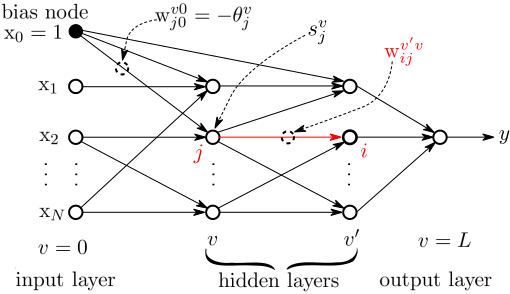
\includegraphics[width=0.99\textwidth]{img/section1_fig14_ij}
         }
     \end{subfigure}
    \end{figure}
    }
\end{frame}

    
    \mode<article>{
    \begin{figure}[h]
        \centering
        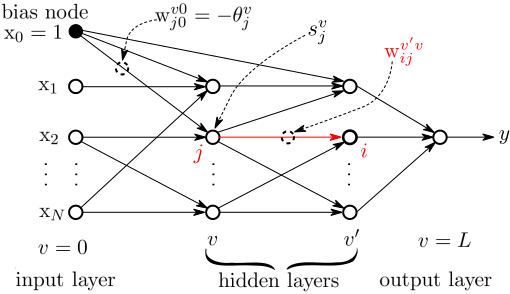
\includegraphics[height=3cm]{img/section1_fig14_ij}
        \caption{Example MLP architecture}
        \label{fig:example_mlp}
    \end{figure}
    
    \eqref{eq:gradient_descent_mlp} shows us how gradients are used for iteratively finding the minimum of the training error.
    The layered structure of an MLP implies that computing the gradient requires a more involved application of the chain rule. The backpropagation algorithm exploits the chain rule to efficiently compute the gradients for an MLP.
    }
    

\mode*

%\section{References}
%\begin{frame}[allowframebreaks] \frametitle{References}
	%\scriptsize
	%\bibliographystyle{plainnat}
	%\bibliography{bibliography}
%\end{frame}

\end{rightcolumn}
\end{paracol}

\end{document}
